\documentclass[12pt,A4,A4pt]{article}

\usepackage{amsmath}
\renewcommand*\familydefault{\sfdefault} 
\usepackage[scaled]{helvet}
\renewcommand\familydefault{\sfdefault} 
\usepackage[T1]{fontenc}
%\usepackage[T1]{fontenc}
%\usepackage{arial} 
%\pagestyle{myheadings}{}
 %\markboth{left head}{right head}
\usepackage{amssymb}
%\usepackage{epsfig}
\usepackage{fancyhdr}
\usepackage{float}
%\usepackage[authoryear,round]{natbib}
\usepackage{apacite}
%\usepackage[sort&compress]{natbib}
\usepackage[pdftex]{graphicx}
\usepackage{color}
\usepackage[brazil]{babel}
\usepackage[utf8]{inputenc}
\usepackage{amsfonts}
\usepackage{textcomp}
\usepackage{tabularx}
\usepackage{multirow}
\usepackage{times}
\usepackage{multicol}
\usepackage{lscape}
\usepackage{subfig}
\usepackage{epstopdf}
\usepackage{setspace}
\usepackage{fancyhdr}
\usepackage{epigraph}
\usepackage{scrextend}
\usepackage[shortlabels]{enumitem}
\usepackage{ragged2e}


%\let\OLDthebibliography\thebibliography
%\renewcommand\thebibliography[1]{\OLDthebibliography{#1} \setlength{\parskip}{0pt}\setlength{\itemsep}{0pt plus 0.3ex}}

%\renewcommand{\chaptermark}[1]{\markboth{\MakeUppercase{#1}}{}}
%\renewcommand{\sectionmark}[1]{\markright{\MakeUppercase{#1}}{}}
\pagestyle{fancy}
\fancyhf{}
\renewcommand{\headrulewidth}{0cm}
%\renewcommand{\footrulewidth}{0}
\usepackage{pdfpages}
\usepackage{stackrel}
\usepackage[left=3cm, right=3cm, top=2.5cm, bottom=2.5cm]{geometry}
\newtheorem{exemplo}{Exemplo}
\newtheorem{definicao}{Definição}
\newtheorem{teorema}{Teorema}
\cfoot{{\fontsize{10pt}{\baselineskip}\selectfont \textbf{8\textsuperscript{o} MCSul / VIII SEMENGO - Universidade Federal do Rio Grande}}}

%%%%%
%tira os numeros da frente do autor
\makeatletter 
\renewcommand\@biblabel[1]{}
\makeatother
%%

\begin{document}
\pretolerance10000

\begin{figure}
\centering
\vspace{-1cm}
\begin{minipage}[c]{\textwidth}
\centering
    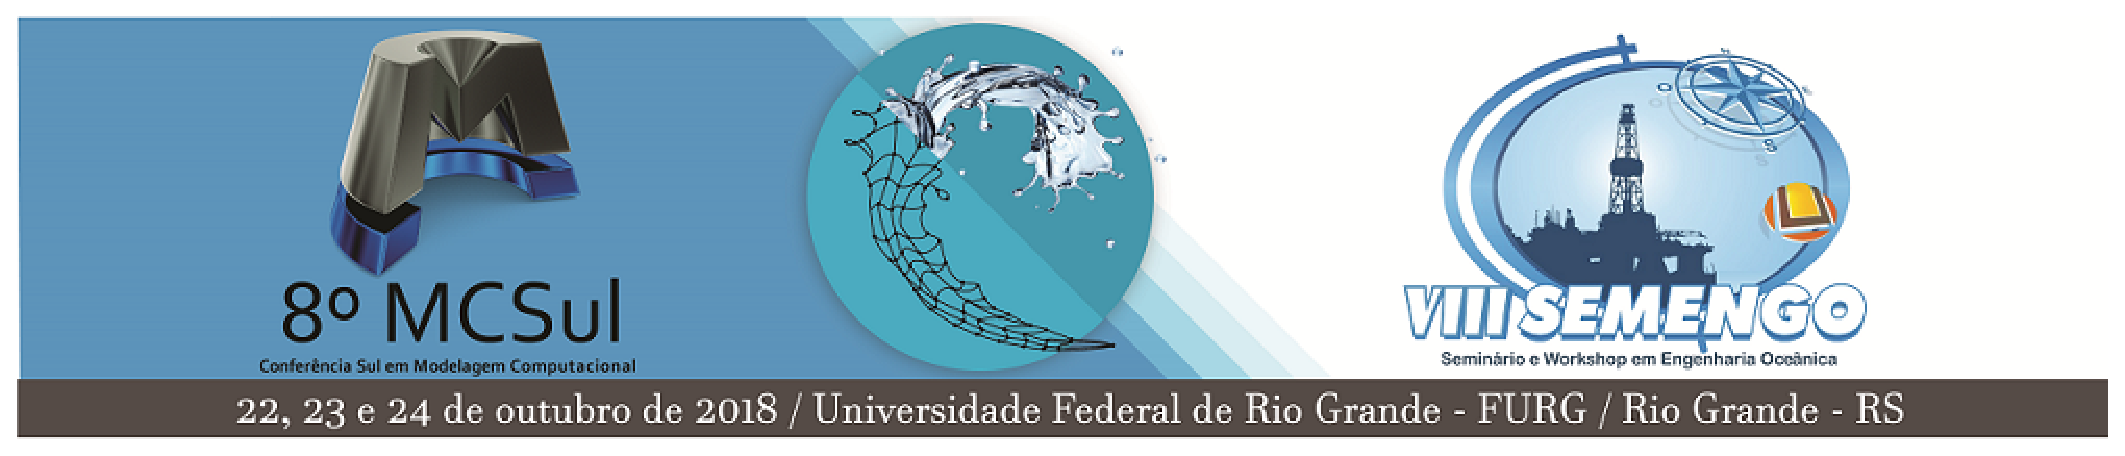
\includegraphics[width=6.2in]{cabecalho.eps}
\end{minipage}
\end{figure}

\begin{center}
\fontsize{16pt}{\baselineskip}\selectfont 
\textbf{{ANÁLISE DO ALGORITMO DE EVOLUÇÃO DIFERENCIAL APLICADO AO DESIGN CONSTRUCTAL DE UMA CAVIDADE EM FORMA DE DUPLO-T}}
\end{center}
\vspace{-0.9cm}
% \begin{center}
% \vspace{0.5cm}
% \textbf{\large{\textit{TÍTULO DO TRABALHO EM INGLÊS}}}
% \end{center}

\begin{flushright}
Gill V. Gonzales\footnote{Mestre, Instituto Federal Sul-Rio-Grandense - Campus Santana do Livramento, RS, Brazil, gillgonzales@ifsul.edu.br.}$^{,2}$

Liércio A. Isold\footnote{Doutor, Universidade Federal do Rio Grande - PPG em Modelagem Computacional, Rio Grande, RS, Brazil, liercioisoldi@furg.br.}

Luiz A. Oliveira Rocha\footnote{Doutor, Universidade do Vale do Rio dos Sinos - PPG em Engenharia Mecânica – São Leopoldo, RS, Brasil luizor@unisinos.br.}

Elizaldo D. dos Santo\footnote{Doutor, Universidade Federal do Rio Grande - PPG em Modelagem Computacional, Rio Grande, RS, Brazil, elizaldosantos@furg.br.}

Antônio J. Silva Neto\footnote{Doutor, Universidade do Estado do Rio de Janeiro, Instituto Politécnico, Nova Friburgo, RJ, Brazil, ajsneto@iprj.uerj.br.}

\end{flushright}

\begin{flushleft}
{\small \setstretch{0.5} \justify
\textbf{Resumo:} Neste trabalho é investigado o desempenho do algoritmo de Evolução Diferencial aplicado à otimização geométrica de um problema de transferência de calor. O problema consiste em uma cavidade em forma de Duplo-T inserida em um sólido com geração de calor constante e uniforme. As laterias do sólido estão em condições adiabáticas e o calor gerado só pode ser removido pela cavidade, a qual é mantida a uma temperatura prescrita. Portanto, a geometria da cavidade influência diretamente a performance térmica do problema. A definição dos graus de liberdade e restrições do problema é realizada através do método de Constructal Design. A otimização geométrica é realizada através do algoritmo de Evolução Diferencial. Neste estudo, são avaliados os parâmetros do algoritmo, tais como o operador de mutação, taxa de cruzamento, fator de amplificação do cálculo diferencial e número de iterações ou avaliação da função objetivo. O número de iteração está relacionado aos parâmetros que configuram o número de gerações e quantidade de indivíduos na população.  O objetivo principal do trabalho é avaliar os parâmetros do algoritmo de Evolução Diferencial e qual a influência na correta reprodução dos efeitos dos graus de liberdade estudados sobre a geometria ótima e performance térmica do problema. Os resultados indicam como mais adequadas as configuração dos parâmetros de taxa de cruzamento e fator de amplificação respectivamente com os seguintes valores 0,7 e 1,5. Estes parâmetros, em conjunto com operador de mutação identificado como de/rand/1/bin, tornaram os resultados do algoritmo mais robustos e necessitando de um menor número de avaliações da função objetivo para a obtenção das geometrias ótimas. A principal contribuição do trabalho é a recomendação de um conjunto de parâmetros adequados que adaptem o algoritmo de Evolução Diferencial ao problema estudado, tornando o algoritmo mais efetivo e robusto para a otimização geométrica do problema estudado.
%contagem de palavras: 298/300

\vspace{0.3cm}

\noindent\textbf{Palavras-chave:} Otimização Geométrica. Transferência de Calor. Constructal Design. Evolução Diferencial.}
\end{flushleft}

% \noindent\textbf{Abstract:} O resumo em inglês apresenta-se logo após o resumo em português. Sugere-se encaminhar o texto para ser traduzido por um profissional. Caso o artigo esteja em inglês, deve haver uma versão do título, resumo e palavras-chave em português ou espanhol.
% \vspace{0.3cm}

% \noindent\textbf{Keywords:} Keywords. Keywords. Keywords. Keywords. Keywords.}

\newpage
 \onehalfspacing
\section{Introdução}

 {\fontsize{12pt}{\baselineskip}\selectfont}
 
\hspace{0.5cm}A pesquisa em cavidades resfriadoras têm início no trabalho de \citeA{Biserni2004}, onde são propostas as formas elementares C e T. Neste trabalho \cite{Biserni2004}, o método de Constructal Design é aplicado para a definição do problema de otimização, assim como a avaliação da influência da geometria sobre a minimização da resistência térmica entre a cavidade e o sólido. O método Constructal Desing é baseado na Teoria Constructal \cite{Bejan}, a qual defende que um princípio físico, a Lei Constructal, determina as formas e estruturas presentes na natureza, sendo a geometria o resultado da otimização da passagem do fluxo em sistemas de escoamento. A Lei Constructal afirma que "Para um sistema de escoamento, animado ou inanimado, evoluir no tempo (sobreviver) é preciso que sua forma e estrutura também evoluam de forma a facilitar a passagem do fluxo"        \cite{Bejan}. Portanto, a geometria é o resultado de um processo de otimização da passagem do escoamento. É importante salientar que o método de Constructal Design (CD) não é o método de otimização. O CD determina os graus de liberdade, restrições e espaço de busca do problema para a avaliação da geometria. Para a otimização geométrica são aplicados métodos de otimização como a Busca Exaustiva ou métodos heurísticas como o Algoritmos Genéticos (AG) e Recozimento Simulado (RS) \cite{Lorenzini2014,Gonzales2015energy}.

\citeA{Biserni2004} concluiu que a cavidade em forma de T é mais eficiente que a primeira forma elementar em C, pois consegue adentrar melhor no domínio computacional investigado. A partir desta observação, formas mais complexas são investigadas na literatura recente \cite{Biserni2007,Lorenzini2011,Lorenzini2014,Biserni2017,Xie2010}. Por exemplo, no trabalho de \citeA{Lorenzini2011} a cavidade proposta em forma de Y, foi até 66\% mais eficiente que a forma elementar T. Portanto, na literatura recente, é possível constatar que formas mais complexas possuem um maior desempenho na minimização da resistência térmica entre o sólido e a cavidade, para o mesmo tipo de problema e mantendo as mesmas restrições. Entretanto, quanto maior a complexidade da cavidade maior é esforço computacional necessário no processo de otimização geométrica, principalmente quando o método de otimização empregado é o método de Busca Exaustiva (BE), quando todas as possibilidades são simuladas. Neste sentido, com a proposta de minimização do esforço computacional e possibilidade de investigar outras características do problema, métodos heurísticos são utilizados no processo de otimização \cite{Lorenzini2014,Gonzales2015energy,Gonzales2017,Biserni2017}.

O uso de métodos heurísticos requer a configuração de parâmetros que controlam o comportamento destes métodos durante o processo de busca pela solução ótima. No trabalho de \citeA{Gonzales2015energy} foi empregado o algoritmo de Recozimento Simulado (RS) para a otimização geométrica da cavidade em forma de Y. Este estudo mostrou como um parâmetro de configuração do método pode influenciar os resultados. O parâmetro analisado foi a função que controla o decaimento da temperatura do RS durante as iterações do algoritmo. Diferentes parâmetros foram investigados e identificados aqueles que levaram ao melhor ou pior desempenho. O parâmetro identificado como $Fast$, por exemplo, apresentou os piores resultados e influenciaria negativamente a avaliação geométrica caso seus resultados fossem utilizados. 

No trabalho de \cite{Gonzales2017} foram comparadas duas diferentes meta-heurísticas, RS e Luus-Jakoola (LJ), e também diferentes versões destes métodos, variando seus parâmetros. Este estudo compara estatisticamente o desempenho dos algorítimos em encontrar a geometria ótima na otimização da cavidade em forma de Duplo-T. Neste estudo, o algoritmo RS, com a função de decaimento de temperatura híbrida identificada como $BoltzExp$, apresenta os melhores resultados entre os métodos investigados. No entanto, no trabalho de \citeA{Gonzales2018}, a mesma análise estatística em encontrar a geometria ótima para o mesmo problema investigado em \cite{Gonzales2017}, foi realizada entre os algortimos de Evolução Diferencial (ED) e RS. Neste estudo, os resultados do algoritmo ED foram superiores aos resultados do algoritmo RS.

Neste artigo, será investigada a aplicação do algoritmo de ED na otimização geométrica da cavidade em forma de Duplo-T. Serão comparados os resultados de diferentes versões do algoritmo ED, configurados com diferentes parâmetros, assim como com diferentes avaliações da função objetivo. 

\section{Modelagem Matemática e Numérica}
\label{modelo}
\hspace{0.5cm}A Figura \ref{figure01} apresenta o sólido em um domínio bidimensional, com a terceira dimensão $W$, perpendicular ao plano da figura. O domínio sólido é representado pela região cinza na Fig. \ref{figure01}, a qual possui uma geração de calor interna constante e uniforme a uma taxa volumétrica dada por $q^{'''}(Wm^{\tiny -3})$. O sólido possui uma condutividade térmica constante $k$. As superfícies externas do sólido estão perfeitamente isoladas (adiabática). Neste caso, o calor só pode ser removido através da cavidade em forma de Duplo-T, que está mantida a uma temperatura mínima $(\theta_{min})$. A temperatura mínima da cavidade representa idealmente o escoamento de um fluido refrigerante em mudança de fase a baixa temperatura escoando pela região da cavidade. Nestes casos, o coeficiente de transferência de calor na parede da cavidade é assumido tão grande que a resistência convectiva pode ser negligenciada em comparação com a resistência condutiva do sólido.

\begin{figure}[h!]
\centering
\includegraphics[width=0.7\linewidth]{imgs/duplo_t.png}
\caption{ {\small Domínio Computacional da Cavidade em Forma de Duplo-T.}}
\label{figure01}
\end{figure}

O objetivo da análise é determinar a geometria ótima ($H/L$, $H_{0}/L_{0}$, $H_{1}/L_{1}$, $H_{2}/L_{2}$ e $S_{1}/H_{0}$) que minimiza a máxima temperatura em excesso adimensional. $(\theta_{max} - \theta_{min})/(q^{'''}A)$. De acordo com o CD esta otimização deve ser submetida as restrições de área total e cavidade, representadas, respectivamente, pelas seguintes equações:

\begin{equation}
A = HL \label{area_total}
\end{equation}
\begin{equation}
A_{c} = A_{0} + 2A_{1} + 2A_{2} \label{area_cavidade}
\end{equation}
A fração da área da cavidade em relação a área total é dada por:
\begin{equation}
\phi_{c} = A_{c}/A \label{fi}
\end{equation}
Para a determinação do campo de temperaturas no domínio sólido, é necessário resolver a equação da condução do calor dada por:
\begin{equation}
\frac{\partial \theta}{\partial \tilde{x}^{2}}+\frac{\partial \theta}{\partial \tilde{y}^{2}}+1=0\label{calor}
\end{equation}

onde as variáveis adimensionais são dadas por:

\begin{equation}
\tilde{\theta} = \frac{\theta - \theta_{min}}{q^{'''}\cdot\frac{A}{k}}\label{tadim}
\end{equation}

\begin{equation}
\tilde{x},\tilde{y},\tilde{H}_{0},\tilde{H}_{1},\tilde{H}_{2},\tilde{L}_{0},\tilde{L}_{1},\tilde{L}_{2},\tilde{H},\tilde{L},\tilde{S}_{1} = \frac{x,y,H_{0},H_{1},H_{2},L_{0},L_{1},L_{2},H,L,S_{1}}{A^{1/2}}\label{vadim}
\end{equation}

Por razões de brevidade, as equações das condições de contorno de fluxo nulo nas superfícies externas ao sólido, bem como, as equações de condições de contorno de temperatura mínima nas paredes da cavidade não são apresentadas, podendo ser vistas no trabalho de  \cite{Gonzales2}.

A forma adimensional das Eqs. \ref{area_total}-\ref{area_cavidade} são representadas pelas seguintes equações:

\begin{equation}
1  = \tilde{H}\tilde{L}\label{total_area_adim}
\end{equation}
\begin{equation}
\phi_{c}=\tilde{H}_{0}\tilde{L}_{0}+2\phi_{1}+2\phi_{2}\label{fi_c}
\end{equation}
\begin{equation}
\phi_{1}=\tilde{H}_{1}\tilde{L}_{1}\label{fi_1}
\end{equation}
\begin{equation}
\phi_{2}=\tilde{H}_{2}\tilde{L}_{2}\label{fi_2}
\end{equation}

O objetivo é minimizar o máximo excesso de temperatura representado pela seguinte equação:

\begin{equation}
\tilde{\theta}_{max}=\frac{\theta_{max}-\theta_{min}}{q^{'''}\cdot\frac{A}{k}}\label{fo}
\end{equation}

Para a determinação da $\tilde{\theta}_{max}$ é necessário a otimização de cinco graus de liberdade ($H/L$, $H_{0}/L_{0}$, $H_{1}/L_{1}$, $H_{2}/L_{2}$ e $S_{1}/H_{0}$) submetidos as restrições de área da cavidade ($\phi_{c}$,$\phi_{1}$ and $\phi_{2}$) e de área total do sólido. Neste artigo, serão otimizados apenas quatro graus de liberdade  ($H/L$, $H_{0}/L_{0}$, $H_{1}/L_{1}$, $H_{2}/L_{2}$ e $S_{1}/H_{0}$).  Em todos os casos a razão $H/L$ será mantida constante ( $H/L$ = 1,0).

A função representada pela Eq. \ref{fo} é resolvida numericamente através da resolução da Eq. \ref{calor} para a determinação dos os campos de temperatura em todo o domínio computacional para diferentes configurações de ($H/L$, $H_{0}/L_{0}$, $H_{1}/L_{1}$, $H_{2}/L_{2}$ e $S_{1}/H_{0}$) e calculando o $\tilde{\theta}_{max}$ para minimizar o seu valor através da variação da configuração geométrica. A solução numérica é dada pela aplicação do método de Elementos Finitos (FEM), baseado em elementos triangulares, desenvolvido no ambiente MATLAB$^{\tiny ®}$, com o pacote PDE (partial-differential-equations) toolbox \citeA{Reddy, Matlab}. A malha é não-uniforme em ambos eixos $x$ e $y$, e varia de uma geometria para outra. O tamanho apropriado da malha é determinado por sucessivos refinamentos de malha (h-adaptativo), aumentando o número de elementos quatro vezes a cada refinamento. Por questões de simplicidade, o teste de malha independente pode ser verificado no trabalho de \cite{Gonzales2}..

\section{Otimização Geométrica}
\label{opt}
\hspace{0.5cm}A otimização geométrica...

\subsection{Constructal Design}
\label{ed}
\hspace{0.5cm}A otimização geométrica...


\subsection{Evolução Diferencial}
\label{ed}
\hspace{0.5cm}A otimização geométrica...

\section{Resultados}
\label{opt}
\hspace{0.5cm}A otimização geométrica...

\section{Conclusão}
\label{opt}
\hspace{0.5cm}A otimização geométrica...

%**********************************************************************************
\section*{Agradecimentos}
\hspace{0.5cm}Agradecimentos e outras seções não numeradas são criadas pela utilização de um asterisco posterior ao comando, \verb|\section*{Agradecimentos}|.

OBS: Parte dos textos utilizados neste modelo para exemplificar seções, quadros, tabelas, etc., foram gentilmente cedidos pela Revista Mundi\footnote{http://periodicos.ifpr.edu.br}, do IFPR.

%**********************************************************************************

\bibliographystyle{apacite}
\bibliography{referencial}

\end{document}